
\chapter*{Úvod}

\addcontentsline{toc}{chapter}{Úvod}

Tato práce se zabývá matematickým modelováním proudění tekutin se zaměřením na hledání optimálního tvaru stěn zejména v problematice úplného kavopulmonálního cévního napojení. V mnoha inženýrských odvětvích jako je např. automobilový nebo letecký průmysl je zapojení procesu optimalizace pro nalezení optimálního tvaru zkoumaného objektu běžnou praxí. V oblasti klinické medicíny však obecně z řady důvodů využití optimalizačních technik stále není tak obvyklé. Pro získání relevantních výsledků je totiž potřeba co nejpřesněji modelovat komplexní proudění krve uvnitř mnohdy složitých geometrií za použití důkladně otestovaných metod. Validace výsledků numerických simulací vůči naměřeným datům je pak také často složitá, jelikož provádění experimentů \textit{in vivo} (v živém organismu) je z~přirozených důvodů velmi obtížné, někdy až nemožné.

Přesto však proces optimalizace tvarů může zejména v kardiochirurgii a cévní chirurgii nacházet velký potenciál \cite{Abraham2005, Weddell2015, Marsden2008}. Vyvinutí optimalizačního procesu použitelného v medicínském prostředí by pro lékaře představovalo \textit{in vitro} (mimo živý organismus) způsob, jak posuzovat chirurgický zákrok v rámci geometrie specifické pro daného pacienta. Navrhování a implantování objektů jako je stent či umělá chlopeň by pak bylo přizpůsobené přímo anatomii pacienta, což může vést ke zlepšeným klinických výsledků, ke snížení rizika pooperačních komplikací a k obecnému zlepšení kvality života pacienta po zákroku \cite{Marsden2008}.

Příkladem konkrétního chirurgického zákroku, kde může proces optimalizace tvaru stěn najít své uplatnění, je tzv. úplné kavopulmonální spojení (anglicky \textit{total cavopulmonary connection}, dále jen TCPC). TCPC se provádí u~dětí, u nichž je diagnostikována tzv. funkčně jediná komora, tj. u~pacientů se závažnou vrozenou srdeční vadou, kvůli které je jejich srdce schopno efektivně využít pouze jednu funkční komoru, a~u~nichž nelze chirurgicky zajistit fungující dvoukomorovou cirkulaci \cite{Chaloup}. Jedná se o~operaci, při které je horní dutá žíla (\textit{vena cava superior}, ozn. \textit{d} na obr. \ref{fig:tcpc}) chirurgicky napojena na plicnici. Také dolní dutá žíla (\textit{vena cava inferior}, ozn. \textit{b} na obr. \ref{fig:tcpc}) je napojena přímo na plicnici (\textit{arteria pulmonalis}, ozn. \textit{a} na obr. \ref{fig:tcpc}) a~to zpravidla pomocí tzv. extrakardiálního konduitu (ozn. \textit{c} na obr. \ref{fig:tcpc}), neboli mimosrdečního kanálu, vytvořeného z cévní protézy \cite{Rubtsova, Delorme}. 

\begin{figure}[h]
	\centering
	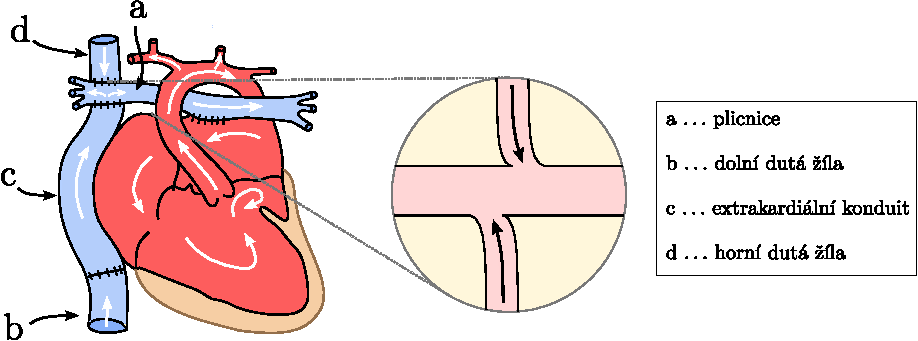
\includegraphics[width=0.84\textwidth]{Images/srdce-zoom.pdf}
	\caption{Schéma úplného kavopulmonálního spojení. Zvětšená část zobrazuje místo napojení mimosrdečního kanálu.}
	\label{fig:tcpc}
	\vspace{-2mm}
\end{figure}

TCPC umožňuje vytvořit funkční oběh krve, vzniklý systém cirkulace je však specifický a je citlivý na vícero faktorů, které nežádoucím způsobem přispívají ke ztrátě energie v systému. To postupně vede k~celkovému selhání systému. Jedná se zejména o vlivy turbulentního proudění a kolize proudů, ke kterým dochází například ve vyústění horní a dolní duté žíly do plicnice. Právě problematika optimálního napojení extrakardiálního konduitu za účelem minimalizace ztráty energie či minimalizace namáhání tkáně může být předmětem procesu optimalizace \cite{Chaloup, vanBake, Wang}. Existuje řada studií zabývající se návrhem optimálního tvaru napojení konduitu, často se však opírají pouze o metodu "pokus-omyl" a~metody optimalizace nepoužívají \cite{Rijnberg2018, Porfiryev2020, Tang2014}.

Pro vytvoření optimalizačního rámce použitelného pro kardiochirurgii při simulování proudění krve je nutné použít k výpočtu hodnot účelové funkce, jež je předmětem minimalizace, efektivní a spolehlivou numerickou metodu. V rámci této práce využijeme k numerickým výpočtům mřížkovou Boltzmannovu metodu (anglicky \textit{lattice Boltzmann method}, dále jen LBM). Poznamenejme, že pro metodu LBM byl použit kód, který je vyvíjený na katedře matematiky FJFI ČVUT v Praze a který byl dle potřeb této práce upraven. Hlavní výhodou LBM je možnost masivní paralelizace na GPU (grafických procesorech), díky čemuž výpočty trvají řádově kratší dobu, než u standardních numerických metod využívaných k~modelování proudění tekutin \cite{PE, Kruger}. Naopak podstatnou nevýhodou LBM z hlediska geometrie hranic je, že pro prostorovou diskretizaci využívá pravidelnou mřížku. To představuje v kontextu této práce výrazný problém, jelikož hranice obtékáných těles nebo hranice cév jsou diskretizovány schodovitě. Proto je část této práce i předchozí bakalářské práce \cite{JB} věnována studiu a implementaci interpolačních okrajových podmínek, které umožňují v rámci diskretizace obtékaných těles zohlednit skutečný tvar jejich hranice. Díky použití těchto okrajových podmínek pak i malá změna tvaru geometrie použité v rámci numerické simulace vede ke změně výsledku získaného pomocí numerické simulace, proto lze v rámci optimalizace využít i např. gradientní optimalizační metody.

Struktura práce je následující. První kapitola se zaměřuje na matematický model proudění tekutin s důrazem na model proudění krve v cévách. Druhá kapitola podrobně rozebírá použitou numerickou metodu LBM. V třetí kapitole je dále rozebrán nástroj vyvinutý pro efektivní parametrizaci a následné automatické generování geometrie. Čtvrtá kapitola obsahuje teorii matematické optimalizace a optimalizační metody použité v této práci, dále je v této kapitole představen navržený použitý optimalizační rámec. Poslední kapitola představuje výsledky provedených numerických simulací. Nejdříve je otestována funkčnost použitého optimalizačního rámce na sérii navržených testovacích úloh s jedním optimalizačním parametrem. Dále je optimalizace testována na složitějších úlohách s více optimalizačními parametry a je mimo jiné zkoumán vliv použité optimalizační metody a volby počátečního odhadu řešení. Jedna ze složitějších úloh zahrnuje zjednodušený 2D model cévní křižovatky vznikající při úplném kavopulmonálním napojení.


